\chapter[Contexto de Serie de Fourier
]{Contexto de Serie de Fourier}
{
\parindent0pt

Según \citet{Arenas2014}, el estudio de las series de Fourier se originó en los trabajos de Joseph Fourier sobre la propagación del calor en cuerpos sólidos. En 1807, presentó su memoria \textit{Mémoire sur la propagation de la chaleur dans les corps solides}, donde analizaba la evolución de la temperatura en función del tiempo. Su trabajo fue clave para el desarrollo de la teoría del análisis de Fourier, que posteriormente consolidó en 1822 con la publicación de \textit{Théorie analytique de la chaleur}, estableciendo los principios para la expansión en series de funciones trigonométricas que representan fenómenos periódicos.
\vspace{10pt}

\begin{figure}[H]
    \centering
    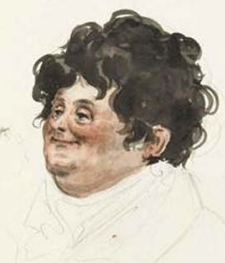
\includegraphics[height=0.15\textheight]{Figures/retrato.png}
    \caption[Retrato caricaturesco de J. Fourier, atribuido a Julien Leopold Boilly]{Retrato caricaturesco de J. Fourier, atribuido a Julien L. Imagen tomada de  \cite{Arenas2014}}
    \label{fig:retrato}
\end{figure}

Las Series de Fourier constituyen una herramienta fundamental en el análisis de funciones, permitiendo representar funciones periódicas como una suma infinita de senos y cosenos. Su estudio se basa en la construcción del espacio \(L^2\) y en la determinación de los coeficientes que conforman la serie. Además, su aplicación se extiende a funciones no periódicas mediante técnicas de extensión y generalización a períodos arbitrarios \citep{DiagoNanez2023}.

\section{Forma Compleja de la Serie de Fourier}
La serie de Fourier puede expresarse en su forma compleja, lo que resulta conveniente en contextos que requieren trabajar con números complejos y simplifica el uso de la Transformada de Fourier \cite{DiagoNanez2023}.  En esta notación, una función \(f(x)\) periódica con período \(T\) se representa como:

\begin{equation} f(x) = \sum_{n=-\infty}^{\infty} c_n e^{i n x}, \end{equation}
\vspace{10pt}

Los coeficientes \(c_n\) se determinan mediante la integral:

\begin{equation} c_n = \frac{1}{T} \int_T f(x) e^{-i n x} , dx \end{equation}

Esta forma compleja de la serie de Fourier permite una interpretación más directa en términos de números complejos y resulta fundamental para la formulación de la Transformada de Fourier \cite{Oppenheim1999, DiagoNanez2023}.

\section{Fórmula Trigonométrica de la Serie de Fourier}

El problema consiste en, dada una función \( f \) de período \( 2\pi \), encontrar su representación en forma de una serie trigonométrica, como se describe en \cite{Arenas2014}. La Serie de Fourier para una función \( f(x) \) en el intervalo \( [-\pi, \pi] \) se expresa de la siguiente manera:

\begin{equation}
\label{eq:fourier}
f(x) = A + \sum_{n=1}^{\infty} a_n \cos(nx) + b_n \sin(nx), \quad \forall x \in T
\end{equation}

En esta ecuación, los coeficientes \( a_0 \), \( a_n \) y \( b_n \) se determinan mediante integrales sobre el intervalo \( T \). Esta representación permite expresar la función \( f(x) \) como una suma infinita de funciones trigonométricas, lo cual facilita el análisis de funciones periódicas.

Los coeficientes \( a_0 \), \( a_n \) y \( b_n \) se calculan mediante las siguientes integrales:
\vspace{10pt}

Coeficiente \( a_0 \):

\begin{equation}
\label{eq:a0Variable}
a_0 = \frac{2}{T} \int_T f(x) \, dx
\end{equation}
\vspace{10pt}

Coeficientes \( a_n \) y \( b_n \):
\vspace{10pt}

\begin{equation}
\label{eq:anVariable}
a_n = \frac{2}{T} \int_T f(x) \cos\left( \frac{2\pi n}{T} x \right) \, dx
\end{equation}

\vspace{10pt}
y
\vspace{10pt}
\begin{equation}
\label{eq:bnVariable}
b_n = \frac{2}{T} \int_T f(x) \sin\left( \frac{2\pi n}{T} x \right) \, dx
\end{equation}
\vspace{10pt}

El procedimiento para obtener el coeficiente \( a_0 \) en la forma trigonométrica de la Serie de Fourier, a partir de la ecuación \eqref{eq:fourier}, es el siguiente. Al integrar esta expresión sobre el intervalo \( T \), y aplicar las propiedades de ortogonalidad de los senos y cosenos, se obtiene:

\[
\int_T f(x) \, dx = \int_T A \, dx + \int_T \sum_{n=1}^{\infty} a_n \cos(nx) + b_n \sin(nx) \, dx 
\]

\begin{equation}
= A \cdot 2\pi + \sum_{n=1}^{\infty} a_n \underbrace{\int_T \cos(nx) \, dx}_{0} + b_n \underbrace{\int_T \sin(nx) \, dx}_{0}
\end{equation}

\[
= A \cdot 2\pi.
\]

Finalmente, tomando \( A = \frac{a_0}{2} \), se obtiene el valor de \( a_0 \) como:

\begin{equation}
a_0 = \frac{1}{\pi} \int_T f(x) \, dx.
\end{equation}
\vspace{10pt}

Para obtener los coeficientes \( a_n \) y \( b_n \), el proceso es análogo. Consiste en multiplicar la ecuación \eqref{eq:fourier} por \( \cos(kx) \) y \( \sin(kx) \), respectivamente, e integrar sobre el intervalo \( T \). Para una derivación detallada de estos coeficientes y una discusión más profunda sobre las series de Fourier, se recomienda consultar \cite{DiagoNanez2023}.

\section{Aplicaciones de la Serie de Fourier}

El análisis de Fourier es una herramienta fundamental en matemáticas e ingeniería, utilizada para descomponer funciones en una suma infinita de senos y cosenos. En particular, la serie de Fourier permite representar funciones periódicas mediante combinaciones de funciones trigonométricas, lo que facilita su estudio y aplicación en diversas áreas del conocimiento \cite{Oppenheim1999}.
\vspace{10pt}

A lo largo de los años, la serie de Fourier ha demostrado ser una herramienta esencial en la resolución de problemas donde la periodicidad y la descomposición en frecuencias juegan un papel clave. Su utilidad se extiende más allá del análisis matemático, permitiendo modelar fenómenos físicos y optimizar procesos en ingenierías. 
\vspace{10pt}

Gracias a su capacidad para transformar funciones complejas en combinaciones de términos sinusoidales, esta técnica se ha convertido en un pilar en múltiples disciplinas.



\subsection{Aplicación en la ciencia}

La serie de Fourier es una herramienta matemática fundamental en las áreas de la ciencia como se muestra a continucación.
\vspace{10pt}

En mecánica cuántica, la serie de Fourier es fundamental para resolver la ecuación de Schrödinger en sistemas periódicos. Su aplicación permite describir la evolución temporal de partículas en potenciales periódicos, como en los cristales cuánticos y los superconductores \cite{griffiths2018introduction}. Además, la transformada de Fourier es utilizada en la representación de estados cuánticos en diferentes bases, lo que facilita la simulación de sistemas cuánticos complejos en computación cuántica \cite{nielsen2010quantum}.
\vspace{10pt}

En astronomía, la serie de Fourier se emplea en la espectroscopia astronómica para descomponer la luz de estrellas y galaxias en componentes espectrales. Esto permite identificar la composición química de cuerpos celestes y analizar efectos como el desplazamiento Doppler en exoplanetas \cite{bracewell2003fourier}. 
\vspace{10pt}

En la radioastronomía, la transformada de Fourier es utilizada en la síntesis de imágenes obtenidas por interferometría, lo que ha permitido la observación de agujeros negros y la detección de ondas gravitacionales \cite{thompson2017interferometry}.
\vspace{10pt}

En ciencia de materiales, la serie de Fourier se aplica en el estudio de estructuras cristalinas. Mediante la difracción de rayos X, los científicos pueden analizar patrones de interferencia que se traducen en series de Fourier para determinar la disposición atómica en materiales sólidos. Esto es esencial para el diseño de nuevos materiales con propiedades específicas, como superconductores o aleaciones de alta resistencia \cite{cullity2014elements}.

En la física, la serie de Fourier es ampliamente utilizada para resolver ecuaciones diferenciales que describen sistemas oscilatorios y ondulatorios. Por ejemplo, en mecánica cuántica, la transformada de Fourier permite representar funciones de onda en el espacio de momentos, lo que es esencial para estudiar partículas en potenciales periódicos, como en los cristales y superconductores \cite{griffiths2018introduction}.
\vspace{10pt}

En la química, la serie de Fourier se utiliza en espectroscopía para analizar las frecuencias de vibración de moléculas. Esto es clave para identificar compuestos químicos y estudiar sus propiedades dinámicas, como en la espectroscopía infrarroja y Raman \cite{banwell1994fundamentals}.


\subsection{Aplicación en la tecnología}

La serie de Fourier es una herramienta matemática en áreas de la tecnología. Sirve para analizar señales en el dominio de la frecuencia y permite optimizar sistemas de telecomunicaciones, mejora la compresión de imágenes y audio, y desarrollar algoritmos en el procesamiento de señales digitales. 
\vspace{10pt}

En el campo de las telecomunicaciones, la serie de Fourier sirve para la modulación y transmisión de señales. Se emplea en técnicas como la multiplexación por división de frecuencia (FDM) y la modulación por división de frecuencia ortogonal (OFDM), utilizadas en sistemas de comunicación inalámbrica como 4G, 5G y Wi-Fi \cite{proakis2001digital}.
\vspace{10pt}

Las series de Fourier también juegan un papel clave en el procesamiento de imágenes digitales. La transformada de Fourier se utiliza en la compresión de imágenes, como en el estándar JPEG, donde permite representar imágenes en términos de sus componentes de frecuencia y eliminar información redundante \cite{gonzalez2017digital}.
\vspace{10pt}

En el campo de la tecnología de audio, la serie de Fourier se utiliza para analizar y procesar señales de sonido. Por ejemplo, en la compresión de archivos de audio (como MP3), la transformada de Fourier permite descomponer la señal en sus componentes frecuenciales, lo que facilita la eliminación de frecuencias no perceptibles por el oído humano y, por tanto, reduce el tamaño del archivo sin perder calidad apreciable \cite{oppenheim2010discrete}.
\vspace{10pt}

En el ámbito de la tecnología médica, la serie de Fourier se aplica en dispositivos de diagnóstico por imagen, como los escáneres de resonancia magnética (MRI). Aquí, la transformada de Fourier convierte las señales captadas en el dominio de la frecuencia en imágenes detalladas del cuerpo humano, lo que permite diagnósticos más precisos y no invasivos \cite{haacke2014magnetic}.
\vspace{10pt}

En la tecnología de energía, la serie de Fourier es fundamental para el análisis de señales en sistemas de potencia. Permite identificar y corregir distorsiones armónicas en la red eléctrica, lo que mejora la calidad de la energía y previene fallos en equipos sensibles \cite{mcgranghan2017power}.

\subsection{Aplicación en la ingeniería}

La serie de Fourier es una herramienta matemática para diversas ramas de la ingeniería. Su capacidad para descomponer señales y analizar su comportamiento en el dominio de la frecuencia mejora el diseño y optimización de sistemas en ingeniería eléctrica, mecánica, civil y biomédica.
\vspace{10pt}

En ingeniería eléctrica, la serie de Fourier se utiliza para analizar y diseñar circuitos de corriente alterna (CA). La representación de señales en el dominio de la frecuencia facilita el estudio del comportamiento de filtros eléctricos, amplificadores y sistemas de comunicación \cite{haykin2001communication}
\vspace{10pt}

En ingeniería mecánica, la serie de Fourier es fundamental en el estudio de vibraciones y el análisis modal de estructuras. Se utiliza para modelar y predecir el comportamiento dinámico de componentes mecánicos sometidos a cargas periódicas, como ejes rotativos, turbinas y motores \cite{inman2001engineering}
\vspace{10pt}

En ingeniería biomédica, la serie de Fourier es esencial para el procesamiento de señales fisiológicas, como electrocardiogramas (ECG) y electroencefalogramas (EEG). Permite la eliminación de ruido en registros médicos y la detección de anomalías en señales biológicas \cite{metin2004biomedical}
\vspace{10pt}

En ingeniería de control, la serie de Fourier es fundamental para el análisis de sistemas dinámicos. Por ejemplo, en el diseño de controladores para robots o vehículos autónomos, la transformada de Fourier ayuda a analizar la respuesta en frecuencia del sistema, lo que permite optimizar su estabilidad y rendimiento \cite{ogata2010modern}.
\vspace{10pt}

En ingeniería civil, la serie de Fourier se utiliza para analizar cargas dinámicas en estructuras, como puentes y edificios. Al estudiar las frecuencias de las fuerzas aplicadas, los ingenieros pueden predecir cómo responderá la estructura a terremotos o vientos fuertes, lo que ayuda a mejorar su diseño y seguridad \cite{chopra2017dynamics}.


\subsection{Aplicación en la Inteligencia Artificial}

La serie de Fourier se ha utilizado en diversos campos, incluida la Inteligencia Artificial. Esto puede ser útil en aplicaciones como el reconocimiento de patrones, el procesamiento de imágenes y la optimización de modelos.
\vspace{10pt}

Las Redes Implícitas Neuronales (INR) utilizan perceptrones multicapa para representar funciones de alta frecuencia en dominios de baja dimensión. Recientemente, estas representaciones han logrado resultados destacados en tareas relacionadas con objetos y escenas 3D complejas \cite{benbarka2021seeing}.
\vspace{10pt}

El análisis armónico, que incluye las series de Fourier, se utiliza para comprender cómo las redes neuronales profundas aprenden tareas complejas. Por ejemplo, investigadores de la Universidad de Rice entrenaron una red neuronal profunda para reconocer flujos complejos de aire o agua y predecir sus cambios en el tiempo \cite{choi2023matematicas}.
\vspace{10pt}

Además, las series de Fourier son esenciales en el procesamiento de señales dentro de la IA, permitiendo la eliminación de ruido, la detección de patrones y la mejora de la calidad de las señales \cite{Oppenheim1999}. Esta técnica es clave en aplicaciones como el reconocimiento de voz, la visión por computadora y la bioinformática, donde la extracción de características relevantes en el dominio de la frecuencia mejora la precisión de los modelos de aprendizaje automático.
\vspace{10pt}

En el análisis de series temporales, la serie de Fourier es empleada para descomponer datos en componentes frecuenciales, lo que ayuda a identificar tendencias y patrones periódicos. Esto es especialmente útil en aplicaciones de predicción, como el pronóstico del tiempo o la detección de anomalías en datos financieros \cite{box2015time}.
\vspace{10pt}

En el aprendizaje profundo (deep learning), la transformada de Fourier se utiliza para acelerar operaciones de convolución en redes neuronales convolucionales (CNN). Aplicando la transformada rápida de Fourier (FFT), es posible reducir la complejidad computacional de estas operaciones, lo que permite entrenar modelos más grandes y complejos de manera eficiente \cite{goodfellow2016deep}.
\vspace{10pt}

En la optimización de modelos de IA, la serie de Fourier se utiliza para analizar y suavizar funciones de pérdida. Esto ayuda a identificar mínimos globales en lugar de mínimos locales, lo que mejora la convergencia de algoritmos de optimización como el descenso de gradiente \cite{boyd2004convex}.


\subsection{Aplicación en el cómputo paralelo}

El cómputo paralelo permite acelerar la ejecución de algoritmos dividiendo tareas en múltiples unidades de procesamiento. La serie de Fourier, junto con su transformada rápida (FFT), es ampliamente utilizada en la optimización de estos algoritmos, reduciendo el tiempo de cómputo en problemas como el análisis de señales, la dinámica de fluidos computacional (CFD) y la inteligencia artificial \cite{vanloan1992computational}.
\vspace{10pt}

En visión por computadora, la serie de Fourier se utiliza para mejorar la eficiencia del procesamiento de imágenes mediante filtrado en el dominio de la frecuencia. La implementación de algoritmos FFT en GPU (Unidades de Procesamiento Gráfico) permite acelerar la detección de bordes, el reconocimiento de patrones y la compresión de imágenes \cite{moreland2003fft}.
\vspace{10pt}

En simulaciones numéricas, como en la dinámica de fluidos computacional (CFD), la serie de Fourier se emplea para resolver ecuaciones en diferencias finitas y para modelar turbulencias \cite{canuto2006spectral}.

\vspace{10pt}

En la optimización de algoritmos paralelos, la serie de Fourier se emplea para diseñar técnicas de descomposición de problemas en subproblemas independientes que pueden resolverse en paralelo. Esto es especialmente útil en aplicaciones de aprendizaje automático distribuido, donde la FFT se utiliza para acelerar operaciones matriciales y de convolución en grandes redes neuronales \cite{goodfellow2016deep}.
\vspace{10pt}

En el análisis de big data, la transformada de Fourier se aplica en el procesamiento paralelo de grandes conjuntos de datos temporales o espaciales. Por ejemplo, en astronomía, la FFT se utiliza para analizar señales de telescopios de manera distribuida, lo que permite procesar petabytes de datos en tiempo récord \cite{bracewell2003fourier}.



}

